% !TEX root = ../main.tex

\section{Voorstelling van het bedrijf} % (fold)
\label{sec:Voorstelling}

\subsection{Het bedrijf} % (fold)
\label{sub:bedrijf}

\lipsum[1]

\begin{figure}[H]
  \label{figure:webrtc}
  \centering
  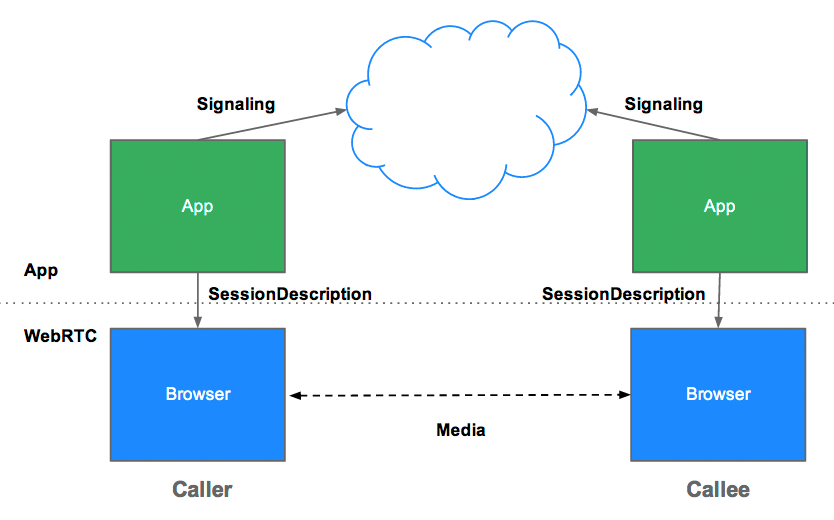
\includegraphics[width=0.8\textwidth]{rtc}
  \caption{Figuur met referentie en bijschrift \cite{voorbeeld-ref}}
\end{figure}

\subsubsection{Werkomgeving}

Citeer bronnen van websites \cite{voorbeeld-ref} en boeken \cite{boek-ref}. Verwijs naar figuren: zie figuur~\ref{figure:webrtc}

\lipsum[1]

